\chapter{Submission 2 ($21^{st}$ March)}
\section{Progress so far}
\begin{itemize}
 \item We have throughly read the paper mentioned in \ref{sec-feasibility}, and implemented the algorithm.
 \item There were some problems in dividing the dataset as the ISEAR dataset mentioned in \ref{sec-dataset}.
 \begin{itemize}
  \item The dataset has a total of 7 emotion classes, but for the sake of simplicity we chose to model only 3 of them.
  \item Out of the 7 classes, 6 are negative emotions (\textbf{sadness, guilt, shame, fear, anger}) and only 1 positive (\textbf{joy}).
  \item We had 2 choices now, either to divide the leftover data for 4 classes into the 2 negative ones, we've chosen (\textbf{anger,sadness}).
  \item Doing this caused some a lot of misclassification, so after some research, we've currently left out 2 emotions - \textbf{guilty,fear}.
 \end{itemize}
 \item Python code to correctly implement the vector space model algorithm mentioned in \ref{subsec-high-level-alg}. We are working collaboratively and have set up a github repo to house all the data, report and code. The link is \url{https://github.com/sm88/mlproject}.
 \item Due to the above mentioned reason for less data, we are looking into some more datasets, mentioned in the paper namely, the Wordnet-Affect dataset and the Semeval dataset.
 \item The wordnet database is not available easily as we need to fill out a form, which after review will enable us to download.
 \item We have throughly cleaned the dataset which had many problems (see figure \ref{fig-clean-dataset}. A few major ones that we solved are:
 \begin{itemize}
  \item Many sentences we of form ``No Response'', which provides no information whatsoever.
  \item There were some scattered braces and square brackets as well as some non-ascii characters, that took a while to catch.
  \item Some sentences were repeated for multiple classes.
 \end{itemize}
 \item We have done some preliminary tests on the training data itself and the results seem promising see table \ref{tab-confusion}.
\end{itemize}
\begin{center}
	\begin{figure}[ht!]
	\label{fig-clean-dataset}	
	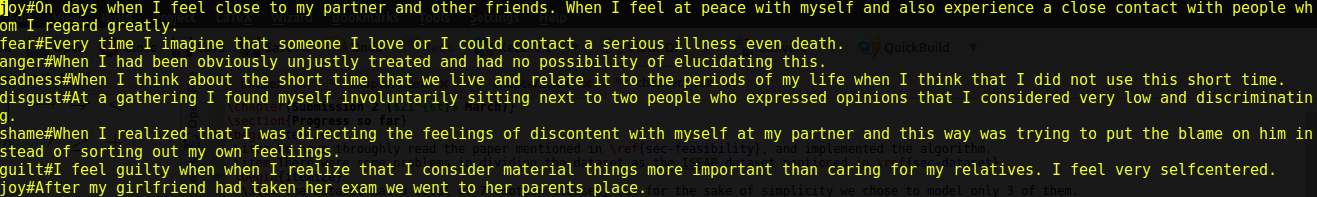
\includegraphics[width=18cm,scale=0.5]{data.png}
	\caption{Cleaned partial ISEAR dataset}
	\end{figure}
\end{center}	
\vspace*{-0.5cm}
\begin{table}[ht!]
  \centering
  \label{tab-confusion}
  \begin{tabular}{c|c|c|c}
  & \textbf{anger} & \textbf{sadness} & \textbf{joy}\\
  \hline
  \textbf{anger} & 1432 & 413 & 318 \\
  \textbf{sadness} & 384 & 2221 & 620 \\
  \textbf{joy} & 28 & 61 & 1001 \\
  \end{tabular}
  \caption{Confusion matrix for training set}
\end{table}
\vspace*{-0.5cm}
\begin{table}[ht!]
  \centering
  \label{tab-accuracy}
  \begin{tabular}{c|c}
  \textbf{Emotion} & \textbf{Accuracy \%} \\
  \hline
  anger & 66 \\
  sadness & 69 \\
  joy & 92
  \end{tabular}
  \caption{Per emotion class accuracy for training set}
\end{table}
\subsection{Other Info}
\begin{itemize}
 \item We believe that with bigger dataset, we'll be able to improve the accuracy of \textbf{anger, sadness} further.
 \item The training time is around a minute and query time is about a second, depending on the length of the sentence.
 \item Our document vectors mentioned in \ref{subsec-high-level-alg} are sparse in nature (total number of words compared to words in a sentence) as a result of which we have excellent opportunities to optimize our implementation.
\end{itemize}
\section{Plan for the rest of the semester}

